\begin{figure*}[htbp]
\setlength{\tabcolsep}{0.5pt} % minimal column spacing
\centering
\begin{tabular}{cccccccccccc}
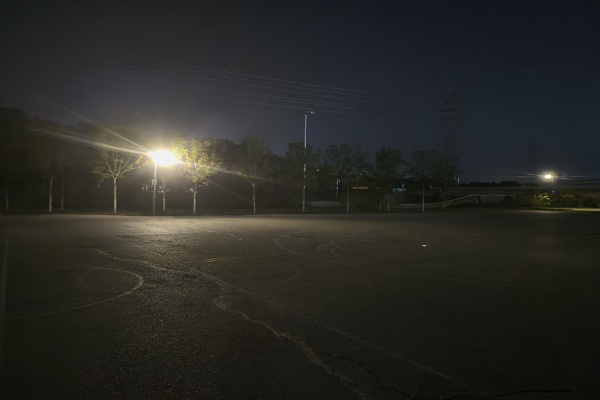
\includegraphics[width = 0.085\linewidth]{figures/compare/night/1.jpg} &
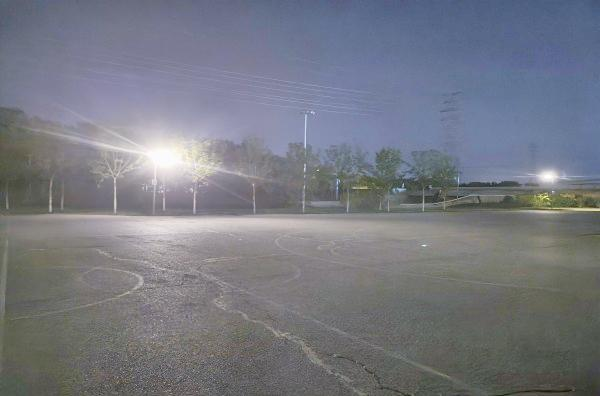
\includegraphics[width = 0.085\linewidth]{figures/compare/zero_dce/1.jpg} &
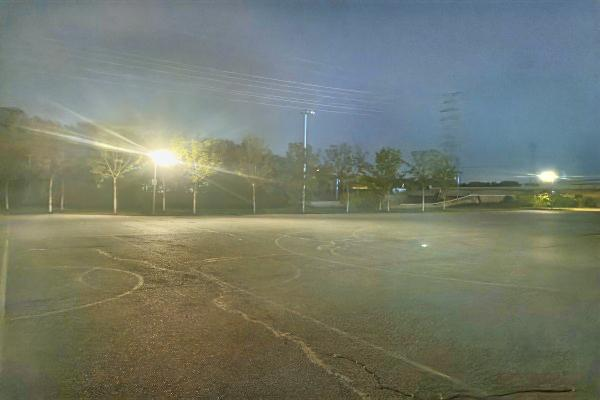
\includegraphics[width = 0.085\linewidth]{figures/compare/enlightengan/1.jpg} &
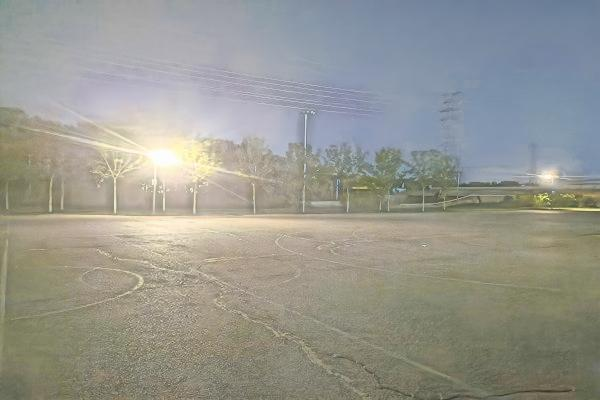
\includegraphics[width = 0.085\linewidth]{figures/compare/cycle_retinex/1.jpg} &
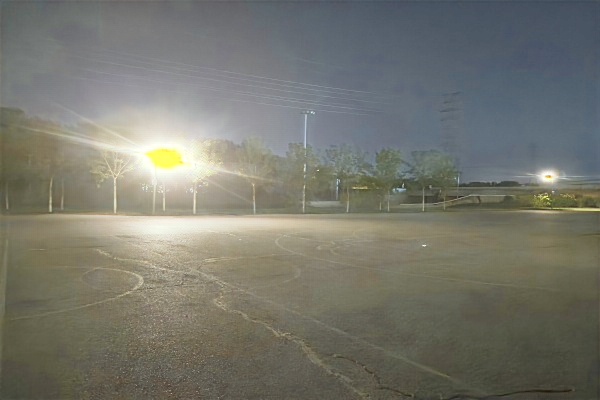
\includegraphics[width = 0.085\linewidth]{figures/compare/retinexformer/1.jpg} &
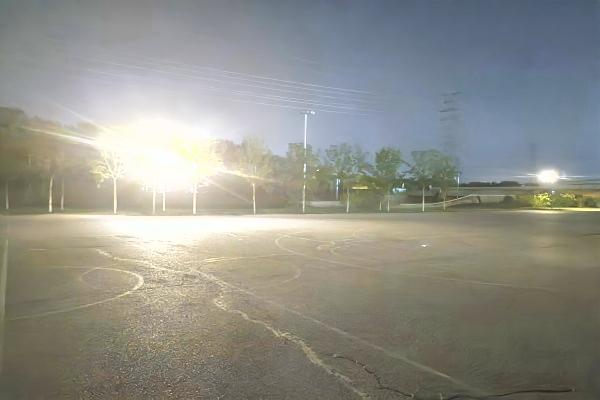
\includegraphics[width = 0.085\linewidth]{figures/compare/hvi_cidnet/1.jpg} &
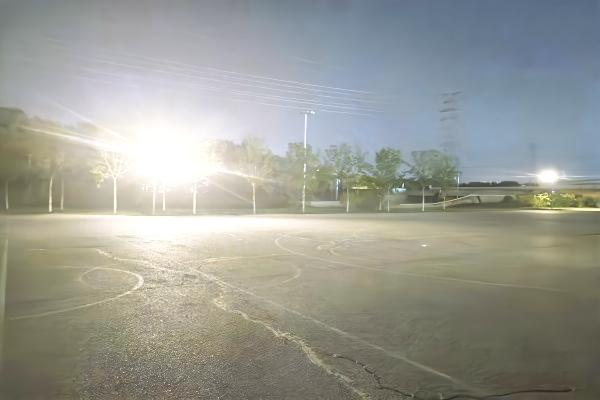
\includegraphics[width = 0.085\linewidth]{figures/compare/reti_diff/1.jpg} &
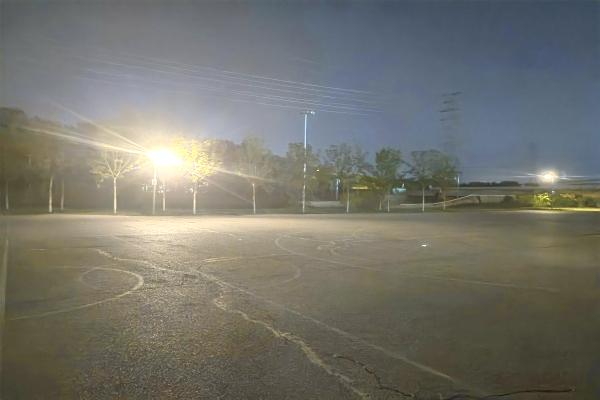
\includegraphics[width = 0.085\linewidth]{figures/compare/multinex/1.jpg} &
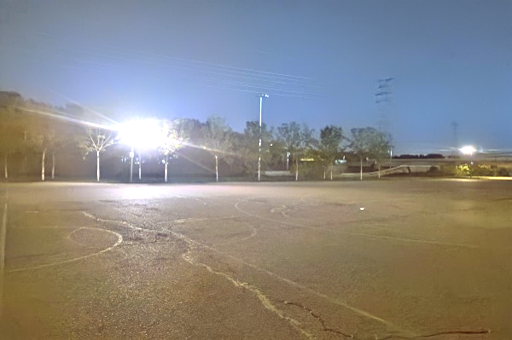
\includegraphics[width = 0.085\linewidth]{figures/compare/cap_vst/1.jpg} &
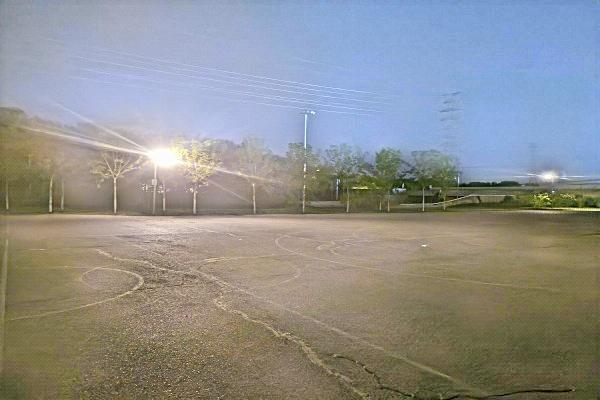
\includegraphics[width = 0.085\linewidth]{figures/compare/ours/1.jpg} &
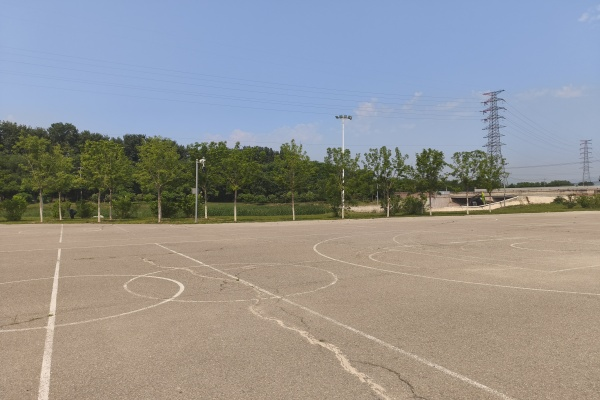
\includegraphics[width = 0.085\linewidth]{figures/compare/day/1.jpg} \\

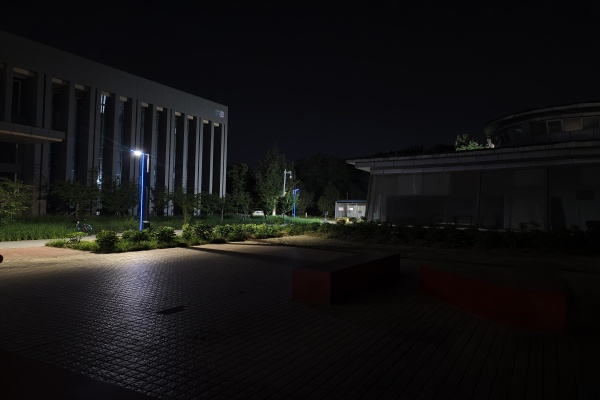
\includegraphics[width = 0.085\linewidth]{figures/compare/night/8.jpg} &
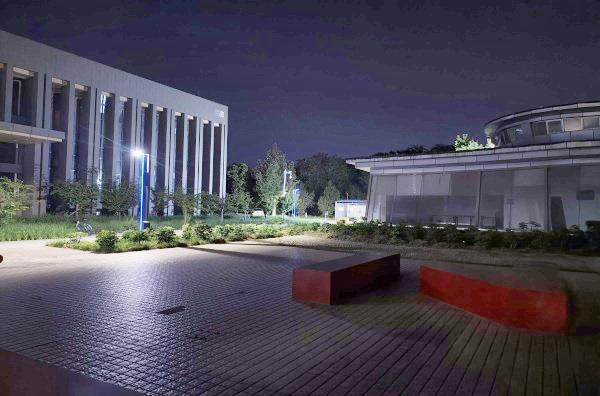
\includegraphics[width = 0.085\linewidth]{figures/compare/zero_dce/8.jpg} &
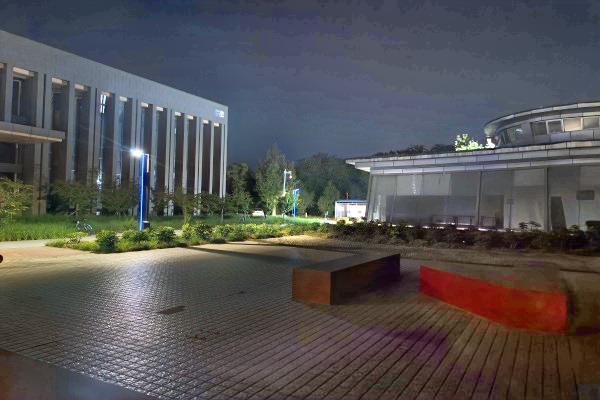
\includegraphics[width = 0.085\linewidth]{figures/compare/enlightengan/8.jpg} &
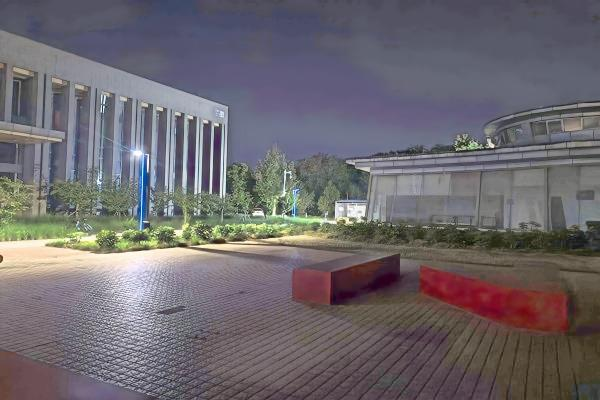
\includegraphics[width = 0.085\linewidth]{figures/compare/cycle_retinex/8.jpg} &
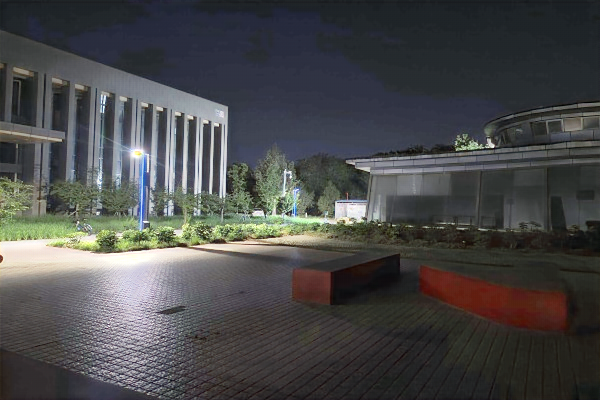
\includegraphics[width = 0.085\linewidth]{figures/compare/retinexformer/8.jpg} &
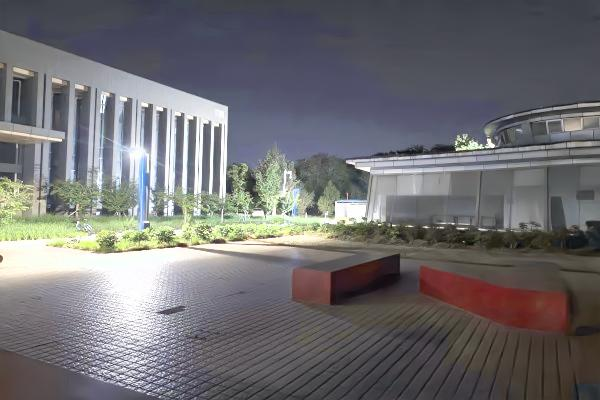
\includegraphics[width = 0.085\linewidth]{figures/compare/hvi_cidnet/8.jpg} &
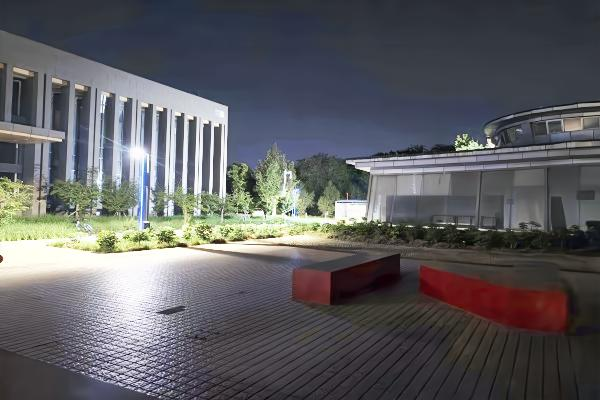
\includegraphics[width = 0.085\linewidth]{figures/compare/reti_diff/8.jpg} &
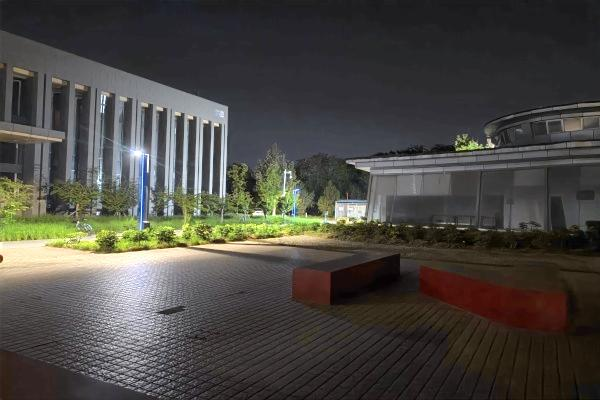
\includegraphics[width = 0.085\linewidth]{figures/compare/multinex/8.jpg} &
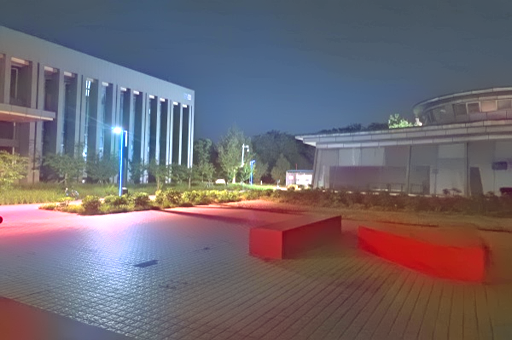
\includegraphics[width = 0.085\linewidth]{figures/compare/cap_vst/8.jpg} &
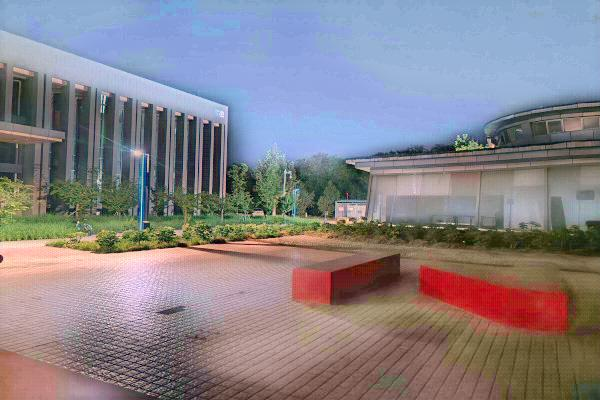
\includegraphics[width = 0.085\linewidth]{figures/compare/ours/8.jpg} &
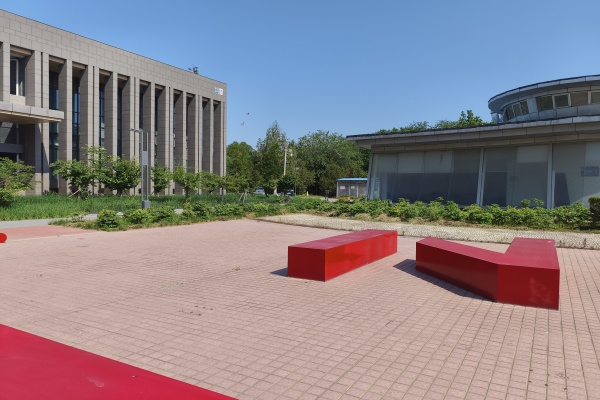
\includegraphics[width = 0.085\linewidth]{figures/compare/day/8.jpg} \\

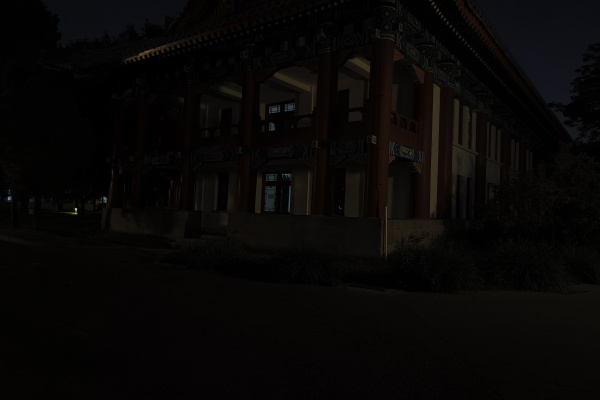
\includegraphics[width = 0.085\linewidth]{figures/compare/night/14.jpg} &
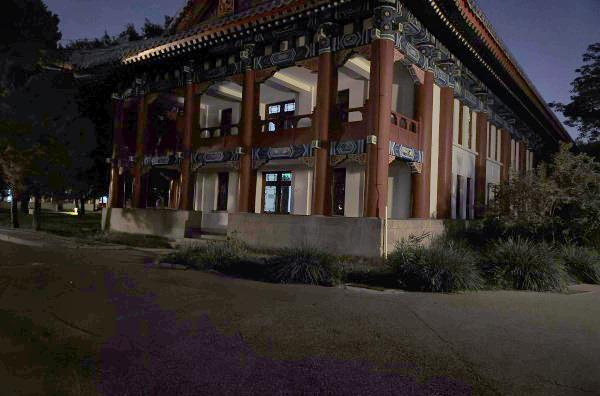
\includegraphics[width = 0.085\linewidth]{figures/compare/zero_dce/14.jpg} &
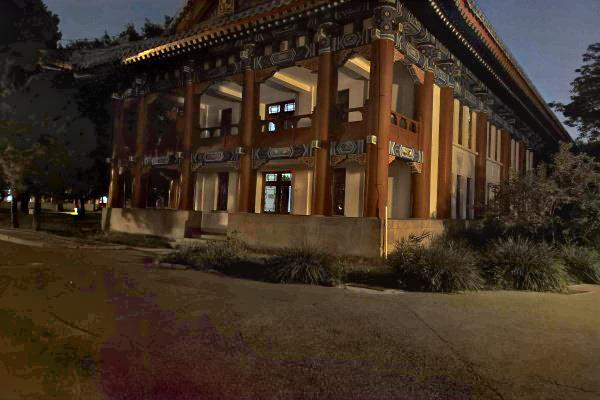
\includegraphics[width = 0.085\linewidth]{figures/compare/enlightengan/14.jpg} &
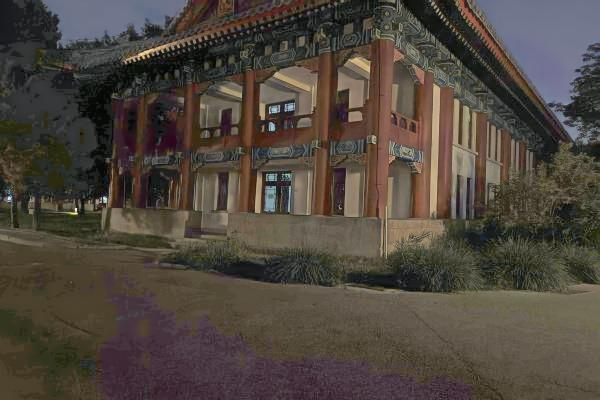
\includegraphics[width = 0.085\linewidth]{figures/compare/cycle_retinex/14.jpg} &
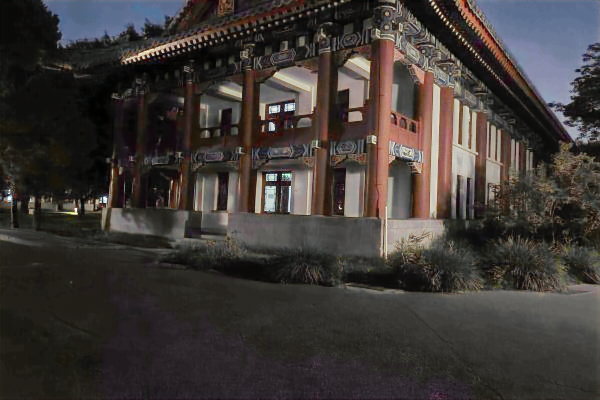
\includegraphics[width = 0.085\linewidth]{figures/compare/retinexformer/14.jpg} &
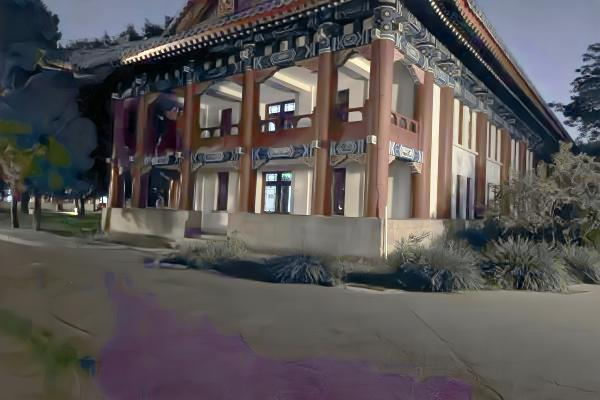
\includegraphics[width = 0.085\linewidth]{figures/compare/hvi_cidnet/14.jpg} &
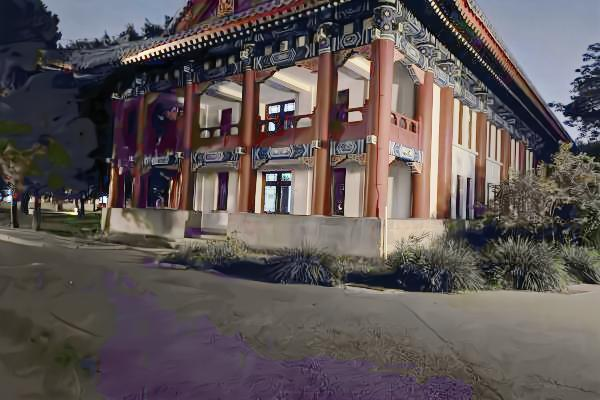
\includegraphics[width = 0.085\linewidth]{figures/compare/reti_diff/14.jpg} &
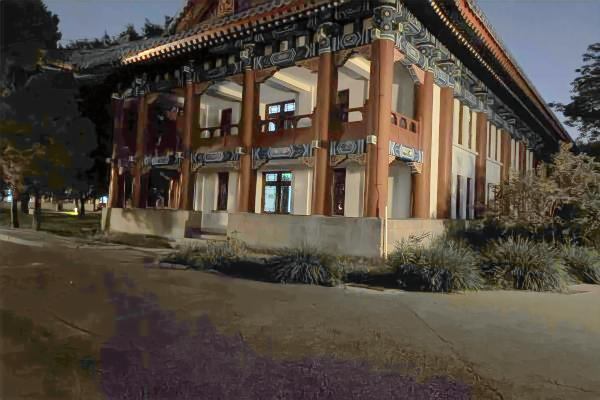
\includegraphics[width = 0.085\linewidth]{figures/compare/multinex/14.jpg} &
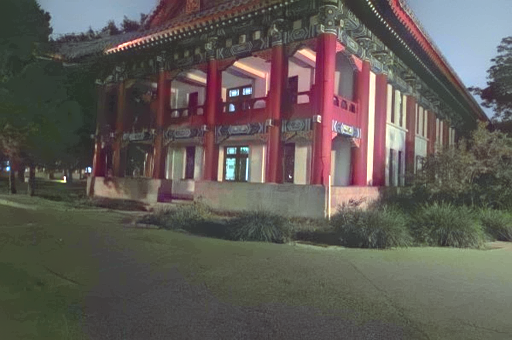
\includegraphics[width = 0.085\linewidth]{figures/compare/cap_vst/14.jpg} &
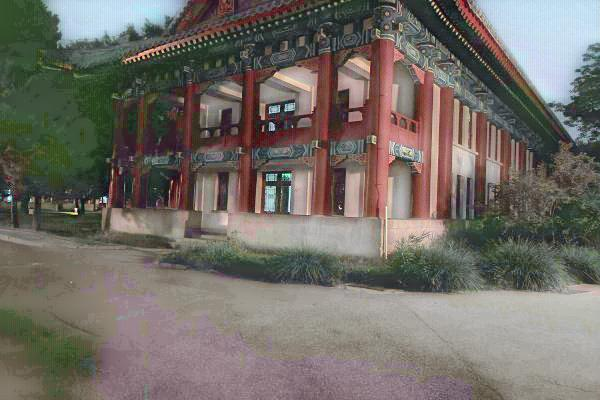
\includegraphics[width = 0.085\linewidth]{figures/compare/ours/14.jpg} &
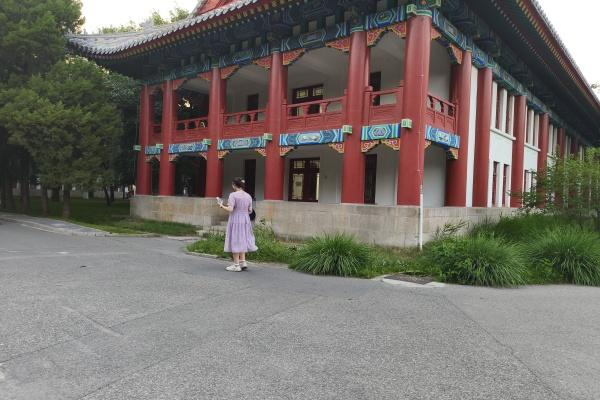
\includegraphics[width = 0.085\linewidth]{figures/compare/day/14.jpg} \\

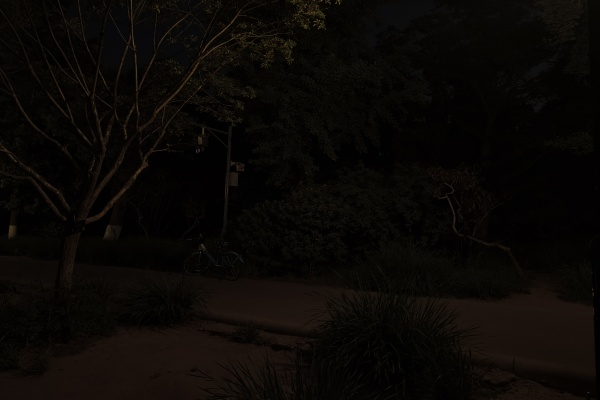
\includegraphics[width = 0.085\linewidth]{figures/compare/night/15.jpg} &
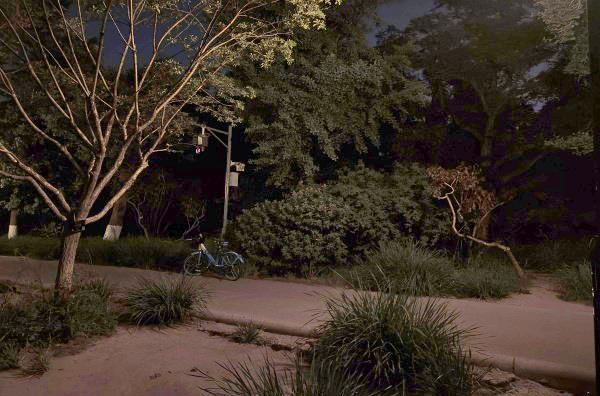
\includegraphics[width = 0.085\linewidth]{figures/compare/zero_dce/15.jpg} &
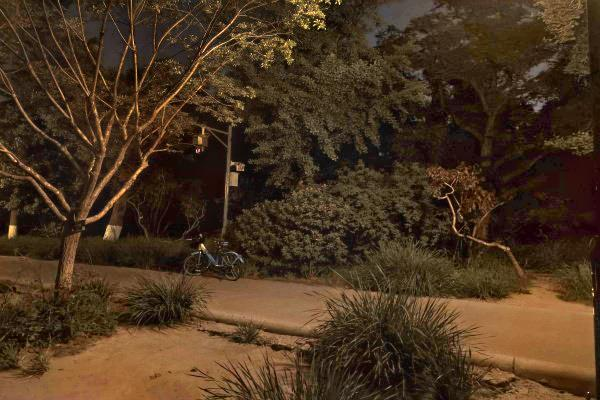
\includegraphics[width = 0.085\linewidth]{figures/compare/enlightengan/15.jpg} &
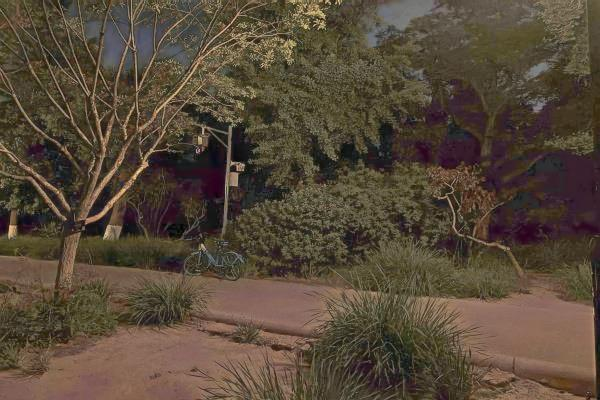
\includegraphics[width = 0.085\linewidth]{figures/compare/cycle_retinex/15.jpg} &
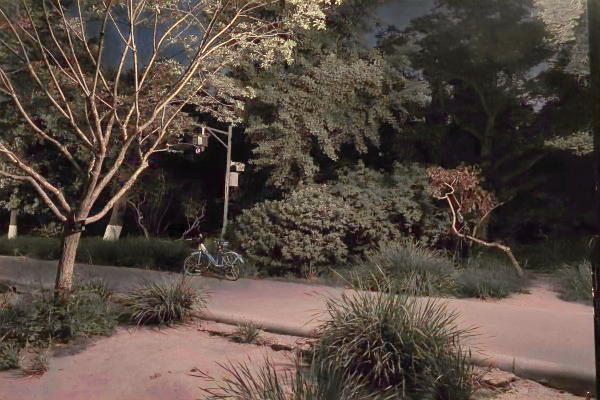
\includegraphics[width = 0.085\linewidth]{figures/compare/retinexformer/15.jpg} &
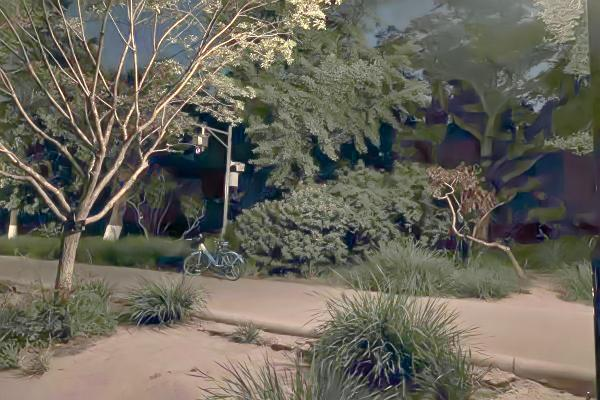
\includegraphics[width = 0.085\linewidth]{figures/compare/hvi_cidnet/15.jpg} &
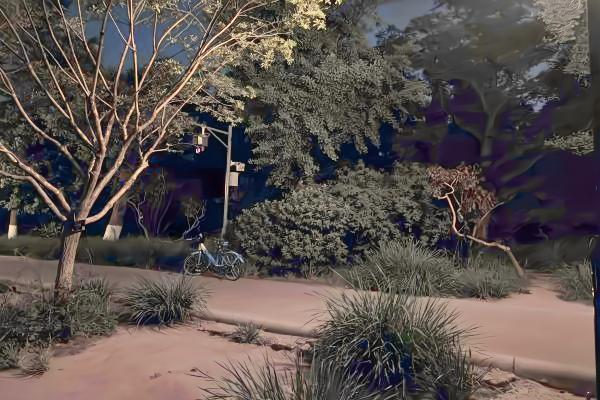
\includegraphics[width = 0.085\linewidth]{figures/compare/reti_diff/15.jpg} &
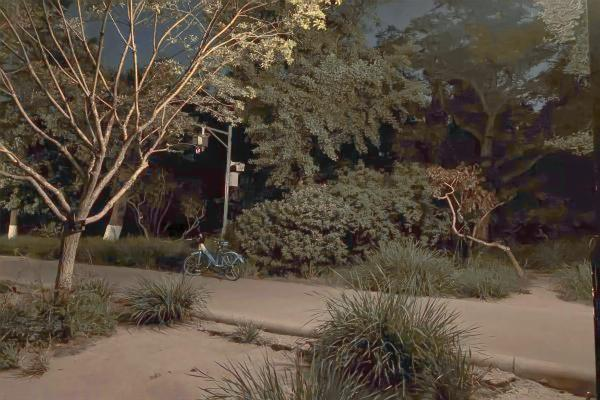
\includegraphics[width = 0.085\linewidth]{figures/compare/multinex/15.jpg} &
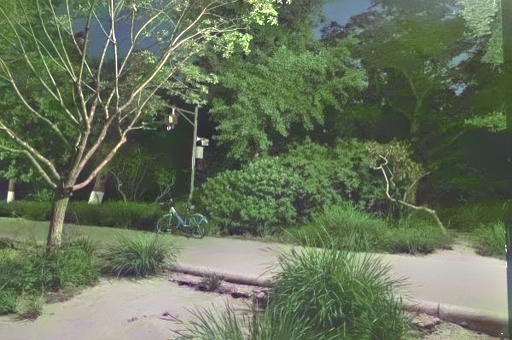
\includegraphics[width = 0.085\linewidth]{figures/compare/cap_vst/15.jpg} &
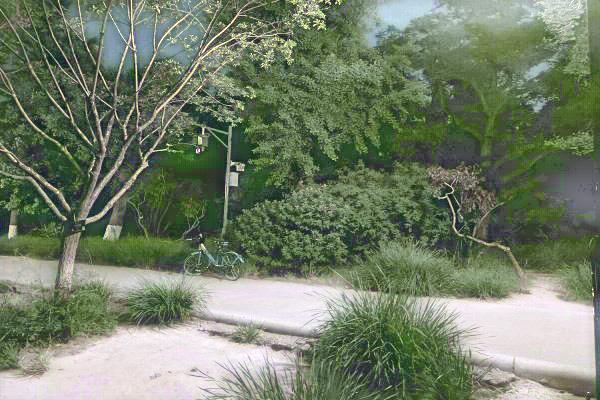
\includegraphics[width = 0.085\linewidth]{figures/compare/ours/15.jpg} &
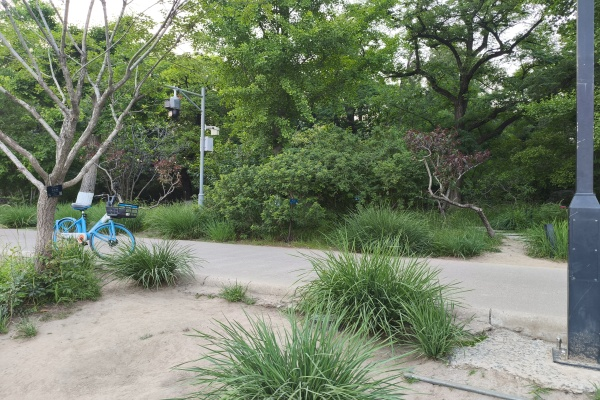
\includegraphics[width = 0.085\linewidth]{figures/compare/day/15.jpg} \\

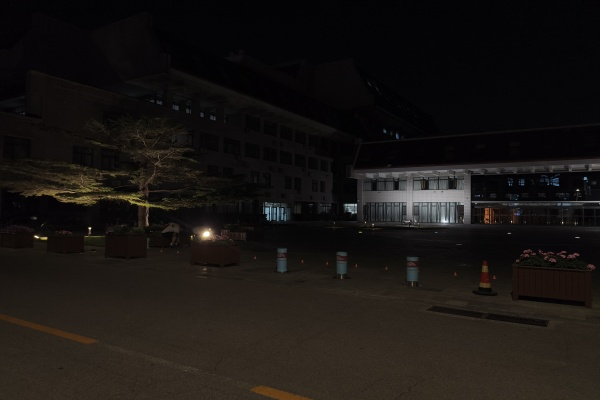
\includegraphics[width = 0.085\linewidth]{figures/compare/night/17.jpg} &
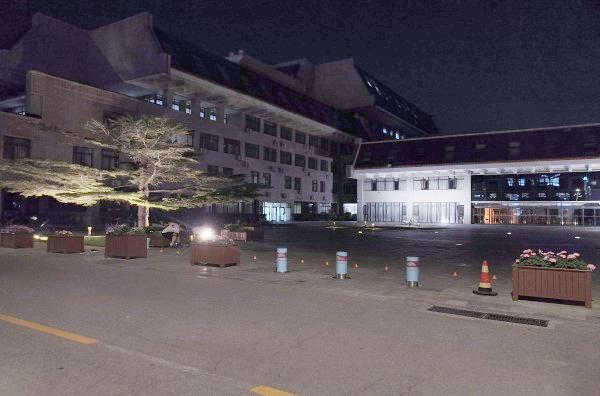
\includegraphics[width = 0.085\linewidth]{figures/compare/zero_dce/17.jpg} &
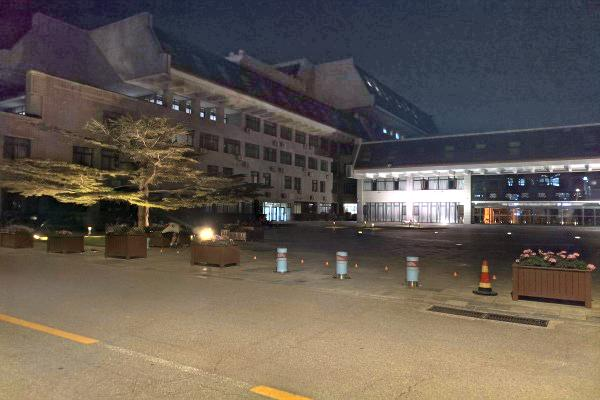
\includegraphics[width = 0.085\linewidth]{figures/compare/enlightengan/17.jpg} &
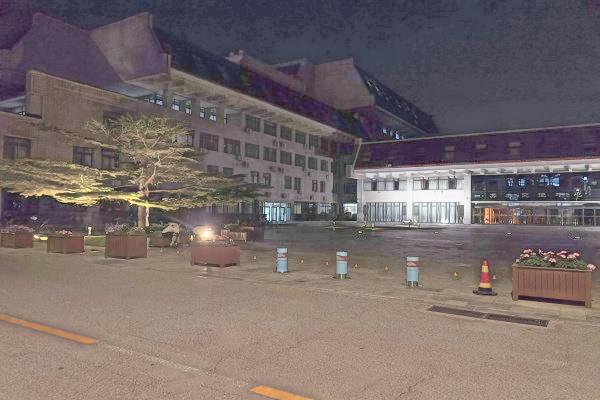
\includegraphics[width = 0.085\linewidth]{figures/compare/cycle_retinex/17.jpg} &
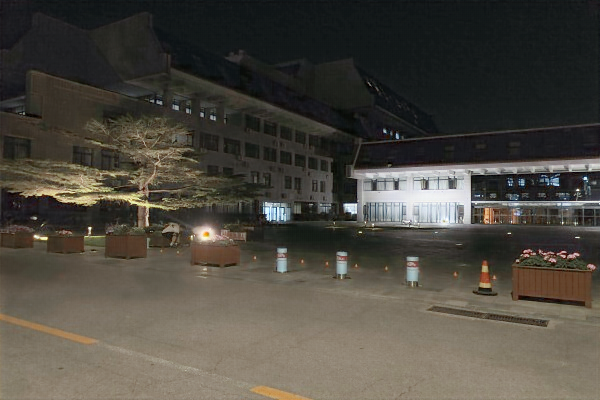
\includegraphics[width = 0.085\linewidth]{figures/compare/retinexformer/17.jpg} &
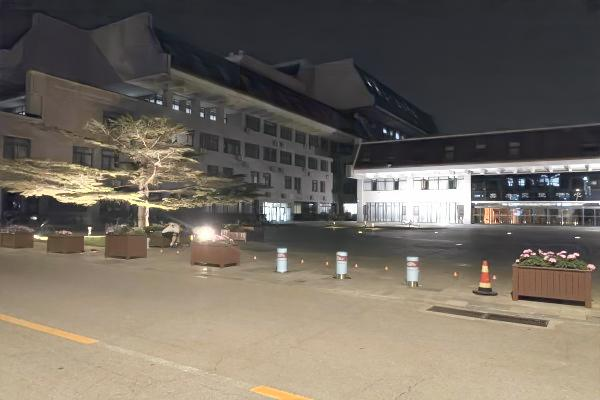
\includegraphics[width = 0.085\linewidth]{figures/compare/hvi_cidnet/17.jpg} &
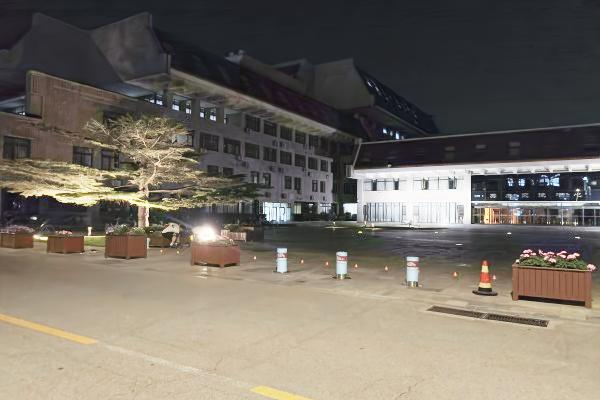
\includegraphics[width = 0.085\linewidth]{figures/compare/reti_diff/17.jpg} &
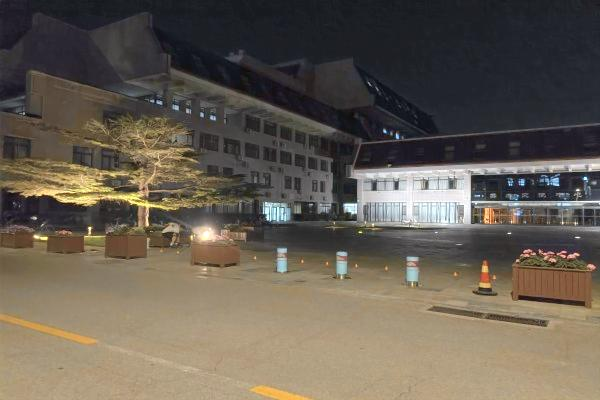
\includegraphics[width = 0.085\linewidth]{figures/compare/multinex/17.jpg} &
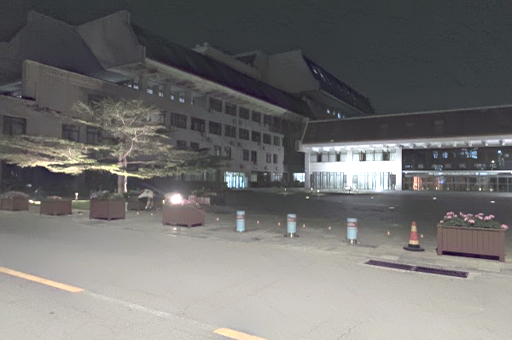
\includegraphics[width = 0.085\linewidth]{figures/compare/cap_vst/17.jpg} &
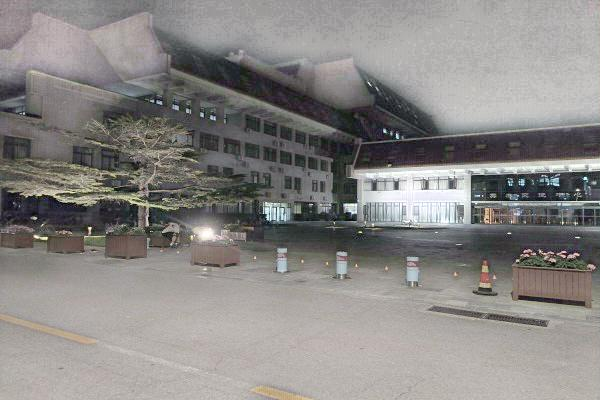
\includegraphics[width = 0.085\linewidth]{figures/compare/ours/17.jpg} &
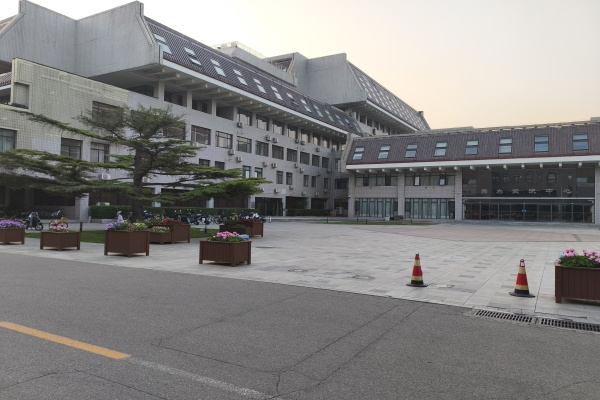
\includegraphics[width = 0.085\linewidth]{figures/compare/day/17.jpg} \\

Night & Zero-DCE++ & EnlightenGAN & Cycle-Retinex & RetinexFormer & HVI-CIDNet & Reti-Diff & Multinex & CAP-VST & Ours (RLTNet) & Reference \\
\end{tabular}
\vspace{.1in}
\caption{Visual comparison on the PKUv2-small validation set. Each row shows one nighttime sample enhanced by seven baselines and our RLTNet, together with the original nighttime input (leftmost) and a scene-consistent daytime reference (rightmost). Daytime references are not pixel-aligned with the night inputs and serve only as a global lighting guide.}\label{fig:compare}
\end{figure*}
